\documentclass[a4paper,11pt]{report}
% -----------------------------------------------------
\usepackage[T1]{fontenc}


\usepackage[utf8]{inputenc}
\usepackage{lmodern}
\usepackage[francais]{babel}
\usepackage{graphicx,color,caption2}
\usepackage{epsfig}
\usepackage{fancyhdr}
\usepackage{textcomp}
\pagestyle{plain}
\usepackage{listings}		% pour incorporer des sources
\usepackage{listingsutf8}		% pour incorporer des sources
\usepackage[francais]{layout}	% pour obtenir le layout
\usepackage{fullpage}		% pour obtenir le layout
\usepackage{makeidx}		% pour créer une table d'index
%\usepackage{shadow}		% pour faire des encadrements
% Modification des marges ------------------------------
\oddsidemargin -4mm 	% Marge de gauche -4mm
\textwidth 17cm 	% Largeur de gauche = 17cm
\parindent 0cm		% Pas d'indentation de paragraphe
% -----------------------------------------------------
\lstset{language={},%C,Assembleur, TeX, tcl, basic, cobol, fortran, logo, make, pascal, perl, prolog, {}
	literate={â}{{\^a}}1 {ê}{{\^e}}1 {î}{{\^i}}1 {ô}{{\^o}}1 {û}{{\^u}}1
		 {ä}{{\"a}}1 {ë}{{\"e}}1 {ï}{{\"i}}1 {ö}{{\"o}}1 {ü}{{\"u}}1
		 {à}{{\`a}}1 {é}{{\'e}}1 {è}{{\`e}}1 {ù}{{\`u}}1 
		 {Â}{{\^A}}1 {Ê}{{\^E}}1 {Î}{{\^I}}1 {Ô}{{\^O}}1 {Û}{{\^U}}1
		 {Ä}{{\"A}}1 {Ë}{{\"E}}1 {Ï}{{\"I}}1 {Ö}{{\"O}}1 {Ü}{{\"U}}1
		 {À}{{\`A}}1 {É}{{\'E}}1 {È}{{\`E}}1 {Ù}{{\`U}}1,
    breaklines=true,    % enleve le débordement de page
	commentstyle=\scriptsize\ttfamily\slshape, % style des commentaires
	basicstyle=\scriptsize\ttfamily, % style par défaut
	keywordstyle=\scriptsize\rmfamily\bfseries,% style des mots-clés
	backgroundcolor=\color[rgb]{.95,.95,.95}, % couleur de fond : gris clair
	framerule=0.5pt,% Taille des bords
	frame=trbl,% Style du cadre
	frameround=tttt, % Bords arrondis 
	tabsize=3, % Taille des tabulations
%	extendedchars=\true, % Incompatible avec utf8 et literate
	inputencoding=utf8,
	showspaces=false, % Ne montre pas les espaces 
	showstringspaces=false, % Ne montre pas les espaces entre ''
	xrightmargin=0.5cm, % Retrait gauche 
	xleftmargin=0.5cm, % Retrait droit
	escapechar=@}  % Caractère d'échappement, permet des commandes latex dans la source
% -----------------------------------------------------

\title{\emph{\textbf{Rapport Project SysG5 :\\ Time Setup}}}
\author{42933 Achetouan Mohammed - 45682 Kardillo Younes}

\begin{document}

\maketitle
\tableofcontents


% Introduction-----------------------------------------------------
\chapter{
  \title{Introduction}
}

L'objectif de ce travail est de créer une application permettant de régler l’heure de différentes machines se trouvant dans un même réseau en utilisant le protocole «\textbf{NTP}».
\\Tout notre script a été fait en utilisant le langage «\textbf{Python}». Afin que notre application se lance dans des meilleures conditions, nous avons opté pour un environnement  virtuel «\textbf{Python3.6.3}».
\\
\\Dans notre application, on donne la possibilité à l’utilisateur de régler l’horloge des machines avec deux méthodes différentes:
\begin{enumerate}
  \item Une machine va régler l’heure des différentes machines du serveur.
  \item Chaque machine demandera à se faire régler son heure à l’aide d’un «\textbf{Cron}».
\end{enumerate}

\section{Concepts théoriques}

\subsection{Protocole $NTP$:}
Le NTP est défini comme un protocole de synchronisation de plusieurs horloges d’un réseau à l’aide d’un ensemble de clients et de serveurs distribués.
Il met à disposition des mécanismes de protocole fondamentaux et nécessaires à la synchronisation de l’heure de différents systèmes jusqu’à une précision de l’ordre de la nanoseconde. D’autre part, il contient des dispositions visant à spécifier la précision et les sources d’erreur possibles de l’horloge système locale ainsi que les propriétés de l’heure de référence.
\footnotemark[1]
\footnotetext[1]{https://www.ionos.fr/digitalguide/serveur/know-how/network-time-protocol}

\subsection{Programme $Cron$:}
cron est un programme qui permet aux utilisateurs des systèmes Unix d’exécuter automatiquement des scripts, des commandes ou des logiciels à une date et une heure spécifiée à l’avance, ou selon un cycle défini à l’avance.
\footnotemark[2]
\footnotetext[2]{https://fr.wikipedia.org/wiki/Cron}

% Installation et configuration-----------------------------------------------------
\chapter{
  \title{Installation et configuration}
}
\section{Installation des différentes dépendances}
Avant de lancer l'application, il vous faudra installer les différentes dépendances.\\Pour ce faire, vous devrez exécuter le script  \textbf{ installationPython} dont voici la commande :
\begin{lstlisting} 
    ./installationPython
\end{lstlisting}
\vspace{3mm}
Une fois l’environnement installé, il faudra activer celui-ci en exécutant cette commande : 
\begin{lstlisting}
    source ~/pythonsProjet-SysG5_TimeSetup/python3.6.3/bin/activate
\end{lstlisting}

\section{Modification des différentes adresses IP}
En fin, il vous faudra insérer les «\textbf{adresses IP}» des machines du serveur dans le fichier \textbf{ressources/src/ipAdresses} sans préciser celle de la machine qui va lancer le script comme ceci :
\\ 
\\ 
$/Projet-SysG5\_TimeSetup/ressources/src/ipAdresses$
\begin{lstlisting}
  192.168.6.130
  192.168.6.131
  192.168.6.132
  192.168.6.133
\end{lstlisting}

\section{Déreglement de l'heure}
Afin que les résultats de notre application soit visible, il est préférable d'ajuster l'heure des autres machines en utilisant cette commande :
\begin{lstlisting} 
    sudo date -s "2 OCT 2006 10:00:00"
\end{lstlisting}

\section{Lancement de l'application}
Une fois tout installés et préparés, il ne vous reste plus qu'à exécuter la commande ci-dessous qui permettra de lancer l’application :
\begin{lstlisting} 
    python ressources/scriptPython/TimeSetup.py
\end{lstlisting}

 % Vue de l'application-----------------------------------------------------
\chapter{
  \title{Vue de l'application}
}
Après toutes les différentes installations et configurations.
\section{Lancement de l'application}
Voici la vue au démmarage de l'application :
\\
\\
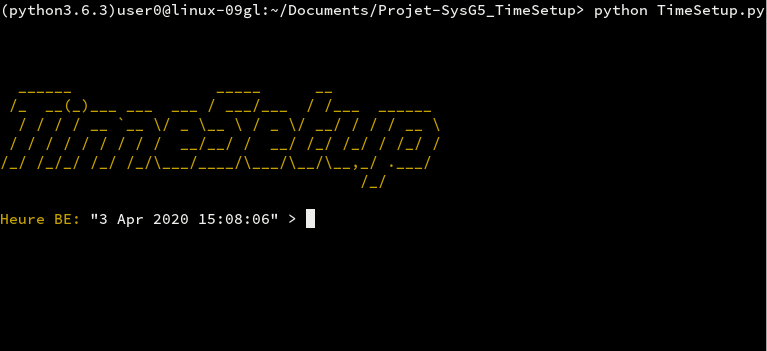
\includegraphics[width=1\textwidth]{ressources/images/screenLancementAPK.PNG}

\newpage
\section{Aide}
Affichage de l'aide :
\\
\\
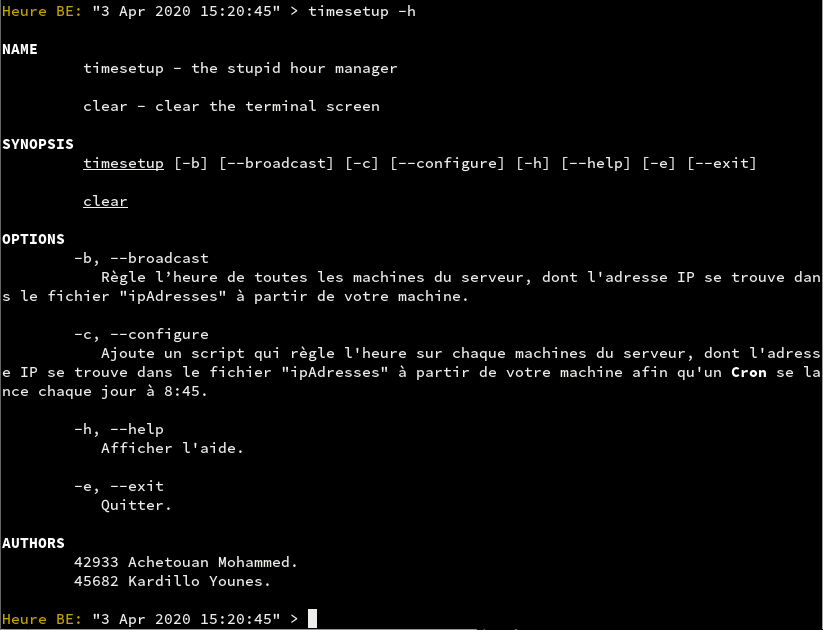
\includegraphics[width=1\textwidth]{ressources/images/screenAideAPK.PNG}

\newpage
\section{Broadcast}
Affichage après exécution de la méthode broadcast :
\\
\\
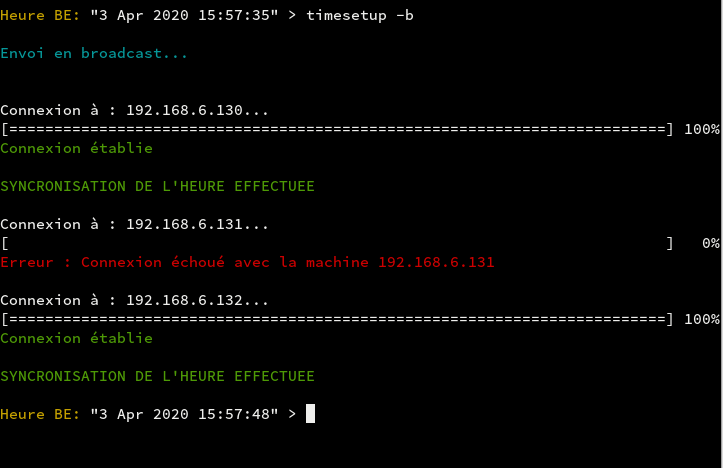
\includegraphics[width=1\textwidth]{ressources/images/screenBroadcastAPK.PNG}
\subsection{Explication :}
Vous pouvez observer sur l'image, que l’application travaille avec 3 machines.
\begin{enumerate}
  \item 192.168.6.130 : \color{green}$Allumée$\color{black}
  \item 192.168.6.131 : \color{red}$Eteinte$\color{black}
  \item 192.168.6.132 : \color{green}$Allumée$\color{black}
\end{enumerate}
La synchronisation a été faite sur les deux machines allumées tant dit que sur celle éteinte, l’application n’a pas pu établir une connexion. Un message d’erreur s’est donc affiché.

\newpage
\section{Configuration}
Affichage après exécution de la méthode configuration :
\\
\\
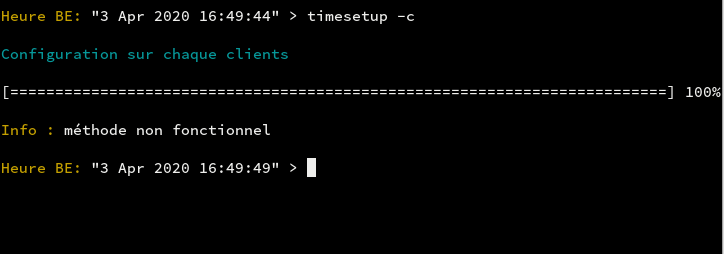
\includegraphics[width=1\textwidth]{ressources/images/screenConfigurationAPK.PNG}
\subsection{Explication :}
Par manque de temps, cette méthode ne fait rien de spéciale.

% Fonctionnement  de l'application-----------------------------------------------------
\chapter{
  \title{Fonctionnement de l'application}
}
Dans cette section, nous nous intéresserons au fonctionnement de l’application, plus particulièrement aux deux méthodes permettant de régler l'horloge des machines.
\section{Méthode 1: Envoie par broadcast}
Lorsque vous entrez la commande suivante:
\begin{lstlisting} 
    timesetup -b
\end{lstlisting}
Ou bien
\begin{lstlisting} 
    timesetup --broadcast
\end{lstlisting}
Vous réglerez l’heure de toutes les machines du serveur, dont l'adresse IP se trouve dans le fichier $ressources/src/ipAdresses$ à partir de votre machine.

\section{Méthode 2: Configuration sur chaque client}
Lorsque vous entrez la commande suivante:
\begin{lstlisting} 
    timesetup -c
\end{lstlisting}
Ou bien
\begin{lstlisting} 
    timesetup --configure
\end{lstlisting}
Vous ajoutez un script qui règle l'heure sur chaque machines du serveur, dont l'adresse IP se trouve dans le fichier $ressources/src/ipAdresses$ afin qu'un «\textbf{Cron}» se lance chaque jour à 8:45.

\section{Aide}
Pour afficher l'aide :
\begin{lstlisting} 
    timesetup -h
\end{lstlisting}
Ou bien
\begin{lstlisting} 
    timesetup --help
\end{lstlisting}

\section{Vider l'affichage}
Pour vider l'invite de commande:
\begin{lstlisting} 
    clear
\end{lstlisting}

\section{Quitter l'application}
Pour quitter l'application, il vous suffit de taper la commande suivante:

\begin{lstlisting} 
    timesetup -e
\end{lstlisting}
Ou bien
\begin{lstlisting} 
    timesetup --exit
\end{lstlisting}

% Explications du TimeSetup.py-----------------------------------------------------
\chapter{
  \title{Explications du fichier TimeSetup.py}
}
Dans cette section, nous expliquerons les variables et les fonctions du fichier $TimeSetup.py$.

\section{Code source}
\lstinputlisting[inputencoding=utf8/latin1]{ressources/scriptPython/TimeSetup.py}


\section{Les variables globales}
	\begin{itemize}
		\item $username$ : représente le nom de l'utilisateur.
		\item $password$ : représente le mot de passe de l'utilisateur.
		\item $root\_Password$ : représente le mot de passe du SuperUser.
		\item $adressIpFilepath$ : représente le path du fichier contenant la liste d'adresse IP.
		\item $heure$ : représente l'heure retourner par la méthode setupTime().
	\end{itemize}
		
\section{Les fonctions}
  \subsubsection{\textbf{setupTime()}:}
  \hspace{0.5cm}
  Cette fonction permet de récuperer l'heure local via le protocole NTP.
  
  \subsubsection{\textbf{configuration()}:}
  \hspace{0.5cm}
  Pour le moment cette fonction ne fait rien de spéciale.
  
  \subsubsection{\textbf{broadcast()}:}
  \hspace{0.5cm}
  Cette fonction récupere les différentes adresses IP du fichier \textbf{ressources/src/ipAdresses}.\\
  Ensuite elle essaye d'établir une connexion avec les machines grâce au protocole de communication SSH. Une fois la connexion établie, elle lance une multitude de commandes permettant de synchroniser l'heure sur les différentes machines.\\
  Pour chaque machine, si la connexion a pu être établie et que la synchronisation a bien été éffectuée alors un message de confirmation est affiché, sinon un message d'erreur apparait expliquant que la connexion a échoué.
  
  \subsubsection{\textbf{displayTitle()}:}
  \hspace{0.5cm}
  Cette fonction affiche le nom du projet avec style.
  
  \subsubsection{\textbf{displayHelp()}:}
  \hspace{0.5cm}
  Cette fonction affiche l'aide de l'application.
  
  \subsubsection{\textbf{clear()}:}
  \hspace{0.5cm}
  Cette fonction permet de vider le terminal.
  
  \subsubsection{\textbf{main()}:}
  \hspace{0.5cm}
  Cette fonction lance l'application et demande à l'utlisateur quelle méthode il souhaite utiliser.
	

% Conclusion-----------------------------------------------------
\chapter{
  \title{Conclusion}
}
Ce projet s’est révélé très enrichissant. En effet, nou avons développé notre prise d’initiative, le respect des délais et le travail en équipe qui sont des aspects essentiels pour notre futur vie de développeur.

De plus, il nous a permis d’appliquer nos connaissances en recherche et en programmation dans un domaine pratique.
\\
\\
Les principaux problèmes, que nous avons rencontrés, sont :
\begin{itemize}
  \item l'adaptation au système d'exploitation $OpenSuse$. 
  \item l’installation d’un environnement $Python3.6.3$ compatible à nos besoins
  \item le paramétrage du protocole de communication $SSH$ entre les machines virtuelles
  \item le manque de matériel (manque de machines pour tester notre application)
  \item perte de temps majeur dû à la configuration des machines virtuelles.
\end{itemize}
\vspace{3mm}
Toutefois, nous avons fait le maximum pour mener à bien ce projet et le rendre agréable pour les utilisateurs.

\end{document}
